\documentclass{beamer}
%
% Choose how your presentation looks.
%
% For more themes, color themes and font themes, see:
% http://deic.uab.es/~iblanes/beamer_gallery/index_by_theme.html
%
\mode<presentation>
{
  \usetheme{default}      % or try Darmstadt, Madrid, Warsaw, ...
  \usecolortheme{default} % or try albatross, beaver, crane, ...
  \usefonttheme{default}  % or try serif, structurebold, ...
  \setbeamertemplate{navigation symbols}{}
  \setbeamertemplate{caption}[numbered]
  \setbeamertemplate{footline}[frame number]
  \setbeamertemplate{itemize items}[circle]
  \setbeamertemplate{theorems}[numbered]
  \setbeamercolor*{structure}{bg=white,fg=blue}
  \setbeamerfont{block title}{size=\normalsize}
}

% \newtheorem{proposition}[theorem]{Proposition}
% \theoremstyle{definition}
% \newtheorem{algorithm}[theorem]{Algorithm}
% \newtheorem{idea}[theorem]{Idea}

\usepackage[english]{babel}
\usepackage[utf8]{inputenc}
\usepackage[T1]{fontenc}
\usepackage{aligned-overset}
\usepackage{alltt}
\usepackage{amsmath}
\usepackage{csquotes}
% \usepackage{multicol}
% \usepackage{stmaryrd}
\usepackage{tabularx}

% \renewcommand\tabularxcolumn[1]{m{#1}}
% \newcolumntype{R}{>{\raggedleft\arraybackslash}X}=

\newcommand\logeq{\mathrel{\vcentcolon\Leftrightarrow}}
\def\code#1{\texttt{\frenchspacing#1}}
\def\padding{\vspace{0.5cm}}
\def\spadding{\vspace{0.25cm}}
\def\b{\textcolor{blue}}
\def\r{\textcolor{red}}
\def\g#1{{\usebeamercolor[fg]{block title example}{#1}}}

% fix for \pause in align
\makeatletter
\let\save@measuring@true\measuring@true
\def\measuring@true{%
  \save@measuring@true
  \def\beamer@sortzero##1{\beamer@ifnextcharospec{\beamer@sortzeroread{##1}}{}}%
  \def\beamer@sortzeroread##1<##2>{}%
  \def\beamer@finalnospec{}%
}
\makeatother

\title[Theoretical Computer Science]{Theoretical Computer Science \\ Regular Languages}
\author{Jonas Hübotter}
\date{}

\begin{document}

\begin{frame}
  \titlepage
\end{frame}

\begin{frame}[allowframebreaks]{Outline}
 \tableofcontents[subsubsectionstyle=hide]
\end{frame}
% \AtBeginSection[]
%   {
%      \begin{frame}[allowframebreaks]{Plan}
%      \tableofcontents[currentsection, sectionstyle=show/hide, hideothersubsections]
%      \end{frame}
%   }

\section{Overview}

\begin{frame}{Overview}
    \begin{block}{Representations of regular languages}\pause
        \begin{itemize}
            \item Right-Linear Grammar (RLG)\pause
            \item Deterministic Finite Automaton (DFA)\pause
            \item Nondeterministic Finite Automaton (NFA)\pause
            \item $\epsilon$-NFA\pause
            \item Regular Expression (Regex)
        \end{itemize}
    \end{block}
\end{frame}

\section{Automata}

\subsection{Deterministic Finite Automaton (DFA)}

\begin{frame}{DFA}
    \begin{definition}
        A \b{deterministic finite automaton (DFA)} $M = (Q, \Sigma, \delta, q_0, F)$\pause\ consists of
        \begin{itemize}
            \item a finite set of \b{states} $Q$\pause;
            \item a (finite) \b{alphabet} $\Sigma$\pause;
            \item a total \b{transition function} $\delta: Q \times \Sigma \to Q$\pause;
            \item an \b{initial state} $q_0 \in Q$\pause; and
            \item a set of \b{terminal (accepting) states} $F \subseteq Q$.
        \end{itemize}
    \end{definition}
\end{frame}

\begin{frame}{DFA}
    \begin{definition}
        The \b{induced transition function} $\hat{\delta}$ of a DFA $M$ is defined by\pause
        \begin{align*}
            \hat{\delta}(q, \epsilon) &= q\pause\\
            \hat{\delta}(q, aw) &= \hat{\delta}(\delta(q,a),w), a \in \Sigma, w \in \Sigma^*.
        \end{align*}\pause
        The language \b{accepted} by $M$ is $L(M) = \{w \in \Sigma^* \mid \hat{\delta}(q_0, w) \in F\}$.
    \end{definition}
\end{frame}

\subsection{Nondeterministic Finite Automaton (NFA)}

\begin{frame}{NFA}
    \begin{definition}
        A \b{nondeterministic finite automaton (NFA)} $N = (Q, \Sigma, \delta, q_0, F)$\pause\ consists of
        \begin{itemize}
            \item $Q, \Sigma, q_0, F$ as defined for DFAs\pause; and
            \item a (partial) \b{transition function} $\delta: Q \times \Sigma \to 2^Q$.
        \end{itemize}
    \end{definition}
\end{frame}

\begin{frame}{NFA}
    \begin{definition}
        The \b{induced transition function} $\hat{\bar{\delta}}$ of a NFA $N$ is defined analogously to $\hat{\delta}$ where\pause
        \begin{align*}
            \bar{\delta}: 2^Q \times \Sigma \to 2^Q, (S, a) \mapsto \bigcup_{q \in S} \delta(q, a).
        \end{align*}\pause
        The language \b{accepted} by $N$ is $L(N) = \{w \in \Sigma^* \mid \hat{\bar{\delta}}(\{q_0\}, w) \cap F \neq \emptyset\}$.
    \end{definition}
\end{frame}

\subsection{NFA $\to$ DFA (determinization)}

\begin{frame}{NFA $\to$ DFA (determinization)}
    \begin{block}{Idea}
        Interpret every reachable subset $S \subseteq 2^Q$ in the NFA $N$ as its own state in the new DFA $M$.\pause\par
        Every state $S$ of $M$ where $S \cap F_N \neq \emptyset$ is an accepting state of $M$.
    \end{block}\pause\padding
    \r{Worst-case exponential growth!}
\end{frame}

\subsection{$\epsilon$-NFA}

\begin{frame}{$\epsilon$-NFA}
    \begin{definition}
        An \b{$\epsilon$-NFA} $N = (Q, \Sigma, \delta, q_0, F)$ is an NFA with a special symbol $\epsilon \neg\in \Sigma$ where
        \begin{align*}
            \delta : Q \times (\Sigma \cup \{\epsilon\}) \to 2^Q.
        \end{align*}\pause
        $\epsilon$-transitions can be executed at any time without reading a symbol.
    \end{definition}
\end{frame}

\subsection{$\epsilon$-NFA $\to$ NFA}

\begin{frame}{$\epsilon$-NFA $\to$ NFA}
    \begin{block}{Idea}
        Given $\epsilon$-NFA $N = (Q, \Sigma, \delta, q_0, F)$\pause\ construct NFA $N' = (Q, \Sigma, \delta', q_0, F')$\pause\ where
        \begin{align*}
            \delta' : Q \times \Sigma \to 2^Q : (q, a) \mapsto \bigcup_{i, j \geq 0} \hat{\delta}(\{q\}, \epsilon^i a \epsilon^j)\pause;
        \end{align*}
        if $\epsilon \in L(N)$ then $F' = F \cup \{q_0\}$ else $F' = F$.
    \end{block}
\end{frame}

\subsection{Product-Construction}

\begin{frame}{Product-Construction}
    \begin{block}{Idea}
        Given DFAs $M_1 = (Q_1, \Sigma, \delta_1, s_1, F_1)$ and $M_2 = (Q_2, \Sigma, \delta_2, s_2, F_2)$\pause\ the \b{product automaton} is $M = (Q_1 \times Q_2, \Sigma, \delta, (s_1, s_2), F_1 \times F_2)$\pause\ where
        \begin{align*}
            \delta &: (Q_1 \times Q_2) \times \Sigma \to Q_1 \times Q_2 \pause\\
                   &: ((q_1, q_2), a) \mapsto (\delta_1(q_1, a), \delta_2(q_2, a)).
        \end{align*}\pause\padding
        For the product automaton $L(M) = L(M_1) \cap L(M_2)$ holds.
    \end{block}
\end{frame}

\subsection{Minimal Automaton}

\begin{frame}{Minimal Automaton}
    For any regular language $L$ there exists a DFA $D$ of minimal size such that $L(D) = L$.\pause
    \begin{block}{Algorithm ($\mathcal{O}(|Q|^2)$ for constant $|\Sigma|$)}
        \begin{enumerate}
            \item remove unreachable states from $q_0$\pause
            \item determine equivalent states\pause
            \item merge equivalent states
        \end{enumerate}
    \end{block}
\end{frame}

\begin{frame}{Equivalent States}
    \begin{definition}
        States $p, q \in Q$ are
        \begin{itemize}
            \item \b{equivalent} if $\forall w \in \Sigma^*.\ \hat{\delta}(p, w) \in F \iff \hat{\delta}(q, w) \in F$\pause;
            \item \b{distinguishable} if they are not equivalent.
        \end{itemize}
    \end{definition}\pause
    \begin{columns}
    \column{0.6\textwidth}
        \begin{block}{Algorithm for finding equivalent states}
            Idea: mark distinguishable states step-by-step.\pause
            \begin{enumerate}
                \item mark all pairs $p, q \in Q$ if $p \in F$ and $q \in Q \setminus F$\pause
                \item while $\exists \text{ unmarked } \{p, q\} \text{ and } \exists a \in \Sigma, \text{ if } \{\delta(p, a), \delta(q, a)\} \text{ is marked, mark } \{p, q\}$
            \end{enumerate}
        \end{block}
    \column{0.4\textwidth}
        \centering
        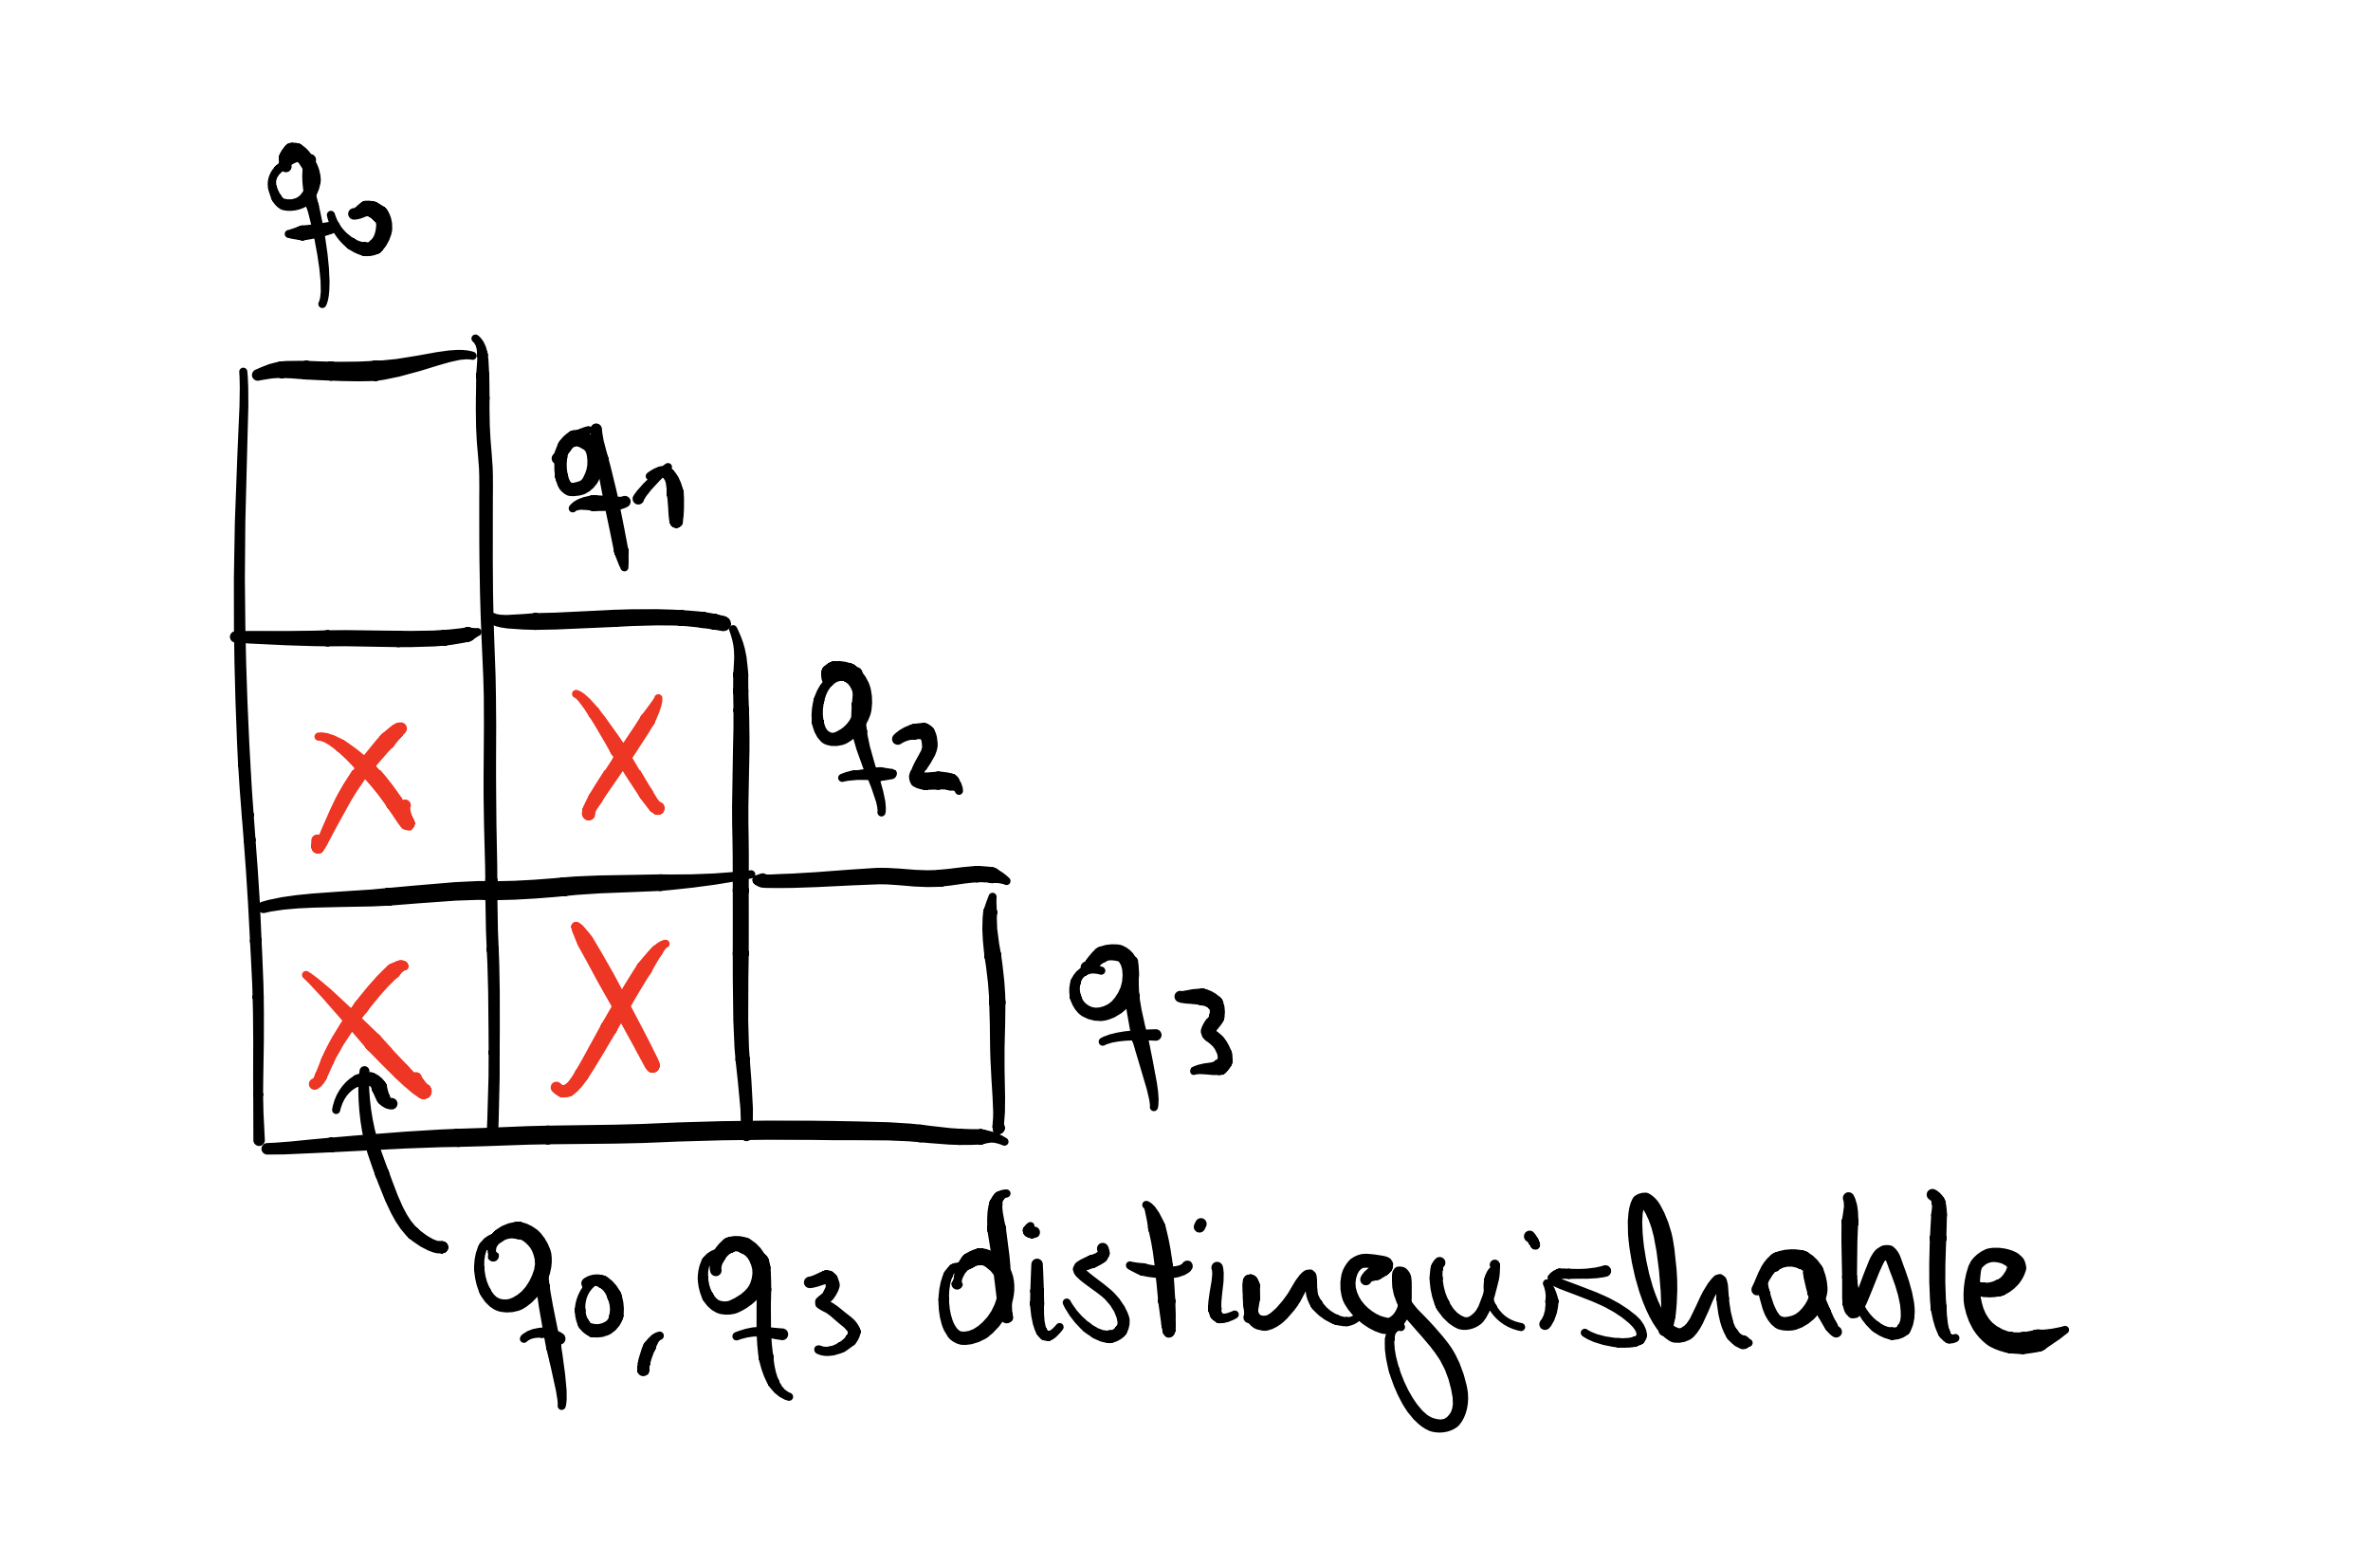
\includegraphics[width=\textwidth]{materials/images/equivalent_states.png}
    \end{columns}
\end{frame}

\subsection{Interlude: Equivalence Relations}

\begin{frame}{Interlude: Equivalence Relations}
    \begin{definition}
        A relation $\sim\ \subseteq A \times A$ is an \b{equivalence relation} if\pause
        \begin{itemize}
            \item $\forall a \in A.\ a \sim a.$ (\b{reflexivity})\pause
            \item $\forall a, b \in A.\ a \sim b \implies b \sim a.$ (\b{symmetry})\pause\ and
            \item $\forall a, b, c \in A.\ a \sim b \land b \sim c \implies a \sim c.$ (\b{transitivity})
        \end{itemize}\pause\par\padding
        $[a]_\sim = \{b \mid a \sim b\}$ is called the \b{equivalence class} of $a$ under $\sim$.\pause\par\padding
        The set of equivalence classes $A/{\sim} = \{[a]_\sim \mid a \in A\}$ is called the \b{quotient set} of $\sim$.
    \end{definition}
\end{frame}

\subsection{Quotient Automaton}

\begin{frame}{Quotient Automaton}
    Observation: the equivalence of states defines an equivalence relation.\pause\par\spadding
    We say $p \equiv_M q$ iff $p$ and $q$ are equivalent states in $M$.\pause\padding
    \begin{definition}
        The collapsed automaton relative to $\equiv_M$ is called \b{quotient automaton}.\pause
        \begin{align*}
            M/{\equiv_M} = (Q/{\equiv_M}, \Sigma, \delta', [q_0]_{\equiv_M}, F/{\equiv_M})
        \end{align*}\pause
        with $\delta'([p]_{\equiv_M}, a) = [\delta(p, a)]_{\equiv_M}$ for $p \in Q, a \in \Sigma$.
    \end{definition}
\end{frame}

\subsection{Canonical Minimal Automaton}

\begin{frame}{Canonical Minimal Automaton}
    \begin{definition}
        The \b{canonical minimal automaton} $M_L$ is a unique minimal automaton for any regular language $L$.\pause
        \begin{align*}
            M_L = (\Sigma^*/{\equiv_L}, \Sigma, \delta_L, [\epsilon]_{\equiv_L}, F_L)
        \end{align*}\pause
        with
        \begin{align*}
            \delta_L([w]_{\equiv_L}, a) &= [wa]_{\equiv_L}\pause \\
            F_L &= \{[w]_{\equiv_L} \mid w \in L\}
        \end{align*}\pause
        It follows that $\hat{\delta}([\epsilon]_{\equiv_L}, w) = [w]_{\equiv_L}$ for $w \in \Sigma^*$,\pause\par
        hence $L(M_L) = L$.
    \end{definition}
\end{frame}

\subsection{Theorem of Mihill-Nerode}

\begin{frame}{Theorem of Mihill-Nerode}
    \begin{theorem}[Theorem of Mihill-Nerode]
        $L \subseteq \Sigma^*$ is regular $\iff$ $\equiv_L$ has finitely many equivalence classes.
    \end{theorem}
\end{frame}

\section{Right-Linear Grammars}

\subsection{DFA $\to$ RLG}

\begin{frame}{DFA $\to$ RLG}
    \begin{block}{Idea}
        Given DFA $M = (Q, \Sigma, \delta, q_0, F)$\pause\ define RLG $G = (Q, \Sigma, P, q_0)$\pause\ with productions $P$:\pause
        \begin{itemize}
            \item $(q_1 \to a q_2) \in P$ iff $\delta(q_1, a) = q_2$\pause;
            \item $(q_1 \to a) \in P$ iff $\delta(q_1, a) \in F$\pause; and
            \item $(q_0 \to \epsilon) \in P$ iff $q_0 \in F$.
        \end{itemize}\pause\padding
        Then, $L(G) = L(M)$.
    \end{block}
\end{frame}

\subsection{RLG $\to$ NFA}

\begin{frame}{RLG $\to$ NFA}
    \begin{block}{Idea}
        Given RLG $G = (V, \Sigma, P, S)$ without the production $S \to \epsilon$\pause,\ define the NFA $N = (V \cup \{q_f\}, \Sigma, \delta, S, \{q_f\})$\pause\ with:
        \begin{itemize}
            \item $Y \in \delta(X, a)$ iff $(X \to aY) \in P$\pause; and
            \item $q_f \in \delta(X, a)$ iff $(X \to a) \in P$.
        \end{itemize}\pause\padding
        Then, $L(N) = L(G)$.
    \end{block}
\end{frame}

\section{Regular Expressions}

\subsection{Definition}

\begin{frame}{Regular Expressions}
    \begin{block}{Syntax}
        \begin{itemize}
            \item $\boldsymbol{\emptyset}$ is a regular expression\pause;
            \item $\epsilon$ is a regular expression\pause;
            \item $\forall a \in \Sigma$, $a$ is a regular expression\pause; and
            \item given regular expressions $\alpha, \beta$, the following are regular expressions:\pause
                \begin{itemize}
                    \item $\alpha \beta$ (\b{concatenation})\pause;
                    \item $\alpha | \beta$ (\b{disjunction})\pause; and
                    \item $\alpha^*$ (\b{repetition}).
                \end{itemize}
        \end{itemize}
    \end{block}
\end{frame}

\begin{frame}{Regular Expressions}
    \begin{block}{Semantics}
        \begin{itemize}
            \item $L(\boldsymbol{\emptyset}) = \emptyset$\pause;
            \item $L(\epsilon) = \{\epsilon\}$\pause;
            \item $L(a) = \{a\}$\pause;
            \item $L(\alpha \beta) = L(\alpha) L(\beta)$\pause;
            \item $L(\alpha | \beta) = L(\alpha) \cup L(\beta)$\pause; and
            \item $L(\alpha^*) = L(\alpha)^*$.
        \end{itemize}
    \end{block}
\end{frame}

\subsection{Interlude: Structural Induction}

\begin{frame}{Interlude: Structural Induction}
    To prove a statement $P$ for an object $\gamma$ that is defined inductively, we use \b{structural induction}.\pause\padding

    Let $\gamma$ be defined by base cases $\alpha_1, \dots, \alpha_k$ and inductive cases $\beta_1, \dots, \beta_l$ with assumptions $a_{i1}, \dots, a_{im_i}$ for $i \in \{1, \dots, l\}$.\pause\padding

    To prove $P$ for all $\gamma$, prove:
    \begin{itemize}
        \item $P(\alpha_i)$ for $i \in \{1, \dots, k\}$\pause; and
        \item $P(a_{i1}) \land \dots \land P(a_{im_i}) \implies P(\beta_i)$ for $i \in \{1, \dots, l\}$.
    \end{itemize}
\end{frame}

\subsection{Regex $\to$ $\epsilon$-NFA (Kleene)}

\begin{frame}{Regex $\to$ $\epsilon$-NFA (Kleene)}
    \begin{columns}
        \column{0.1\textwidth}
        $\boldsymbol{\emptyset}$
        \column{0.6\textwidth}
        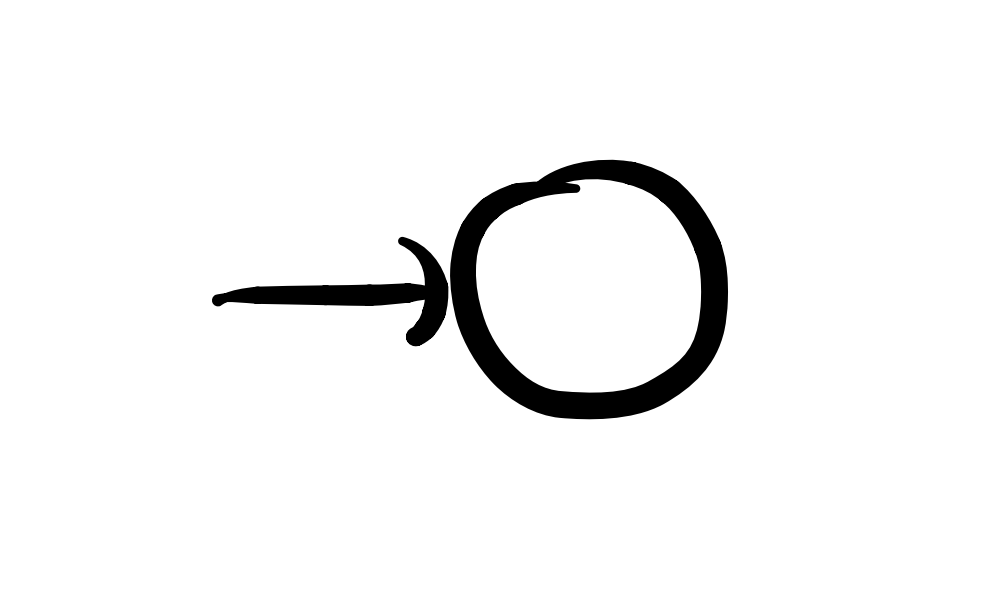
\includegraphics[width=2cm]{materials/images/regex_to_nfa_emptyset.png}
    \end{columns}\pause
    \begin{columns}
        \column{0.1\textwidth}
        $\epsilon$
        \column{0.6\textwidth}
        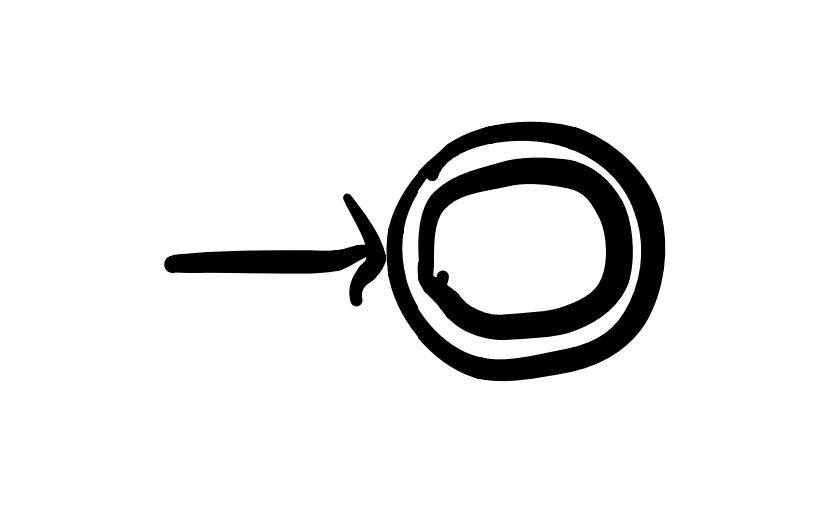
\includegraphics[width=2cm]{materials/images/regex_to_nfa_epsilon.png}
    \end{columns}\pause
    \begin{columns}
        \column{0.1\textwidth}
        $a$
        \column{0.6\textwidth}
        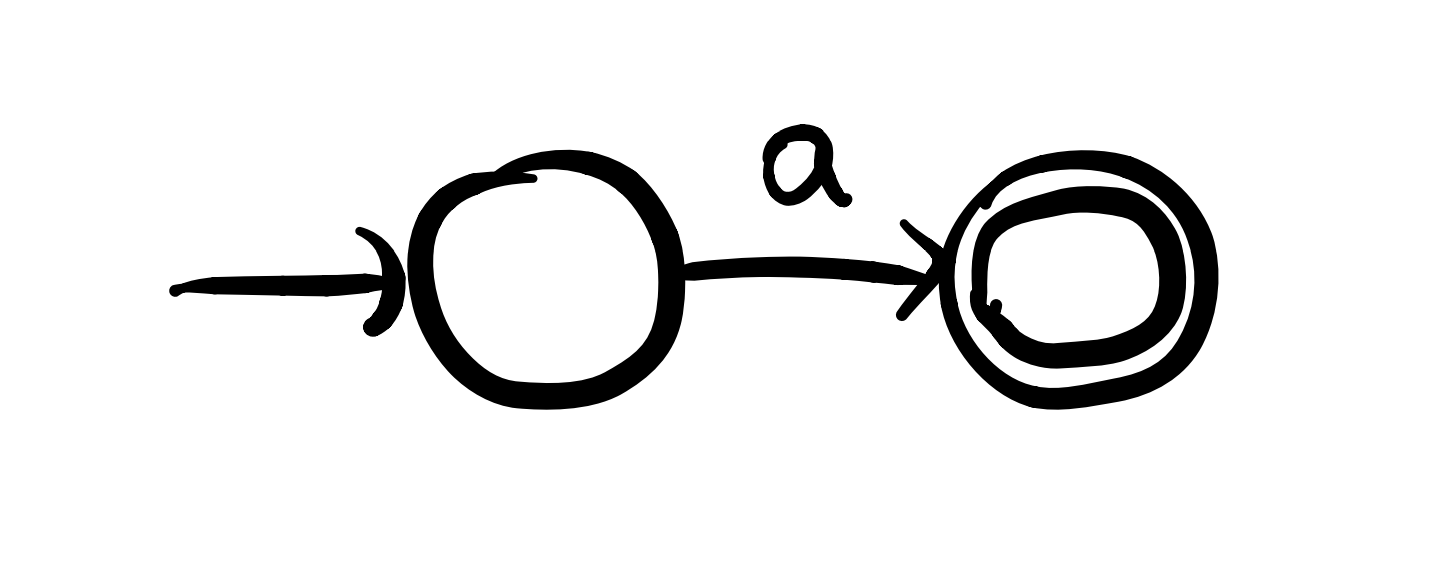
\includegraphics[width=3.5cm]{materials/images/regex_to_nfa_symbol.png}
    \end{columns}\pause
    \begin{columns}
        \column{0.1\textwidth}
        $\alpha \beta$
        \column{0.6\textwidth}
        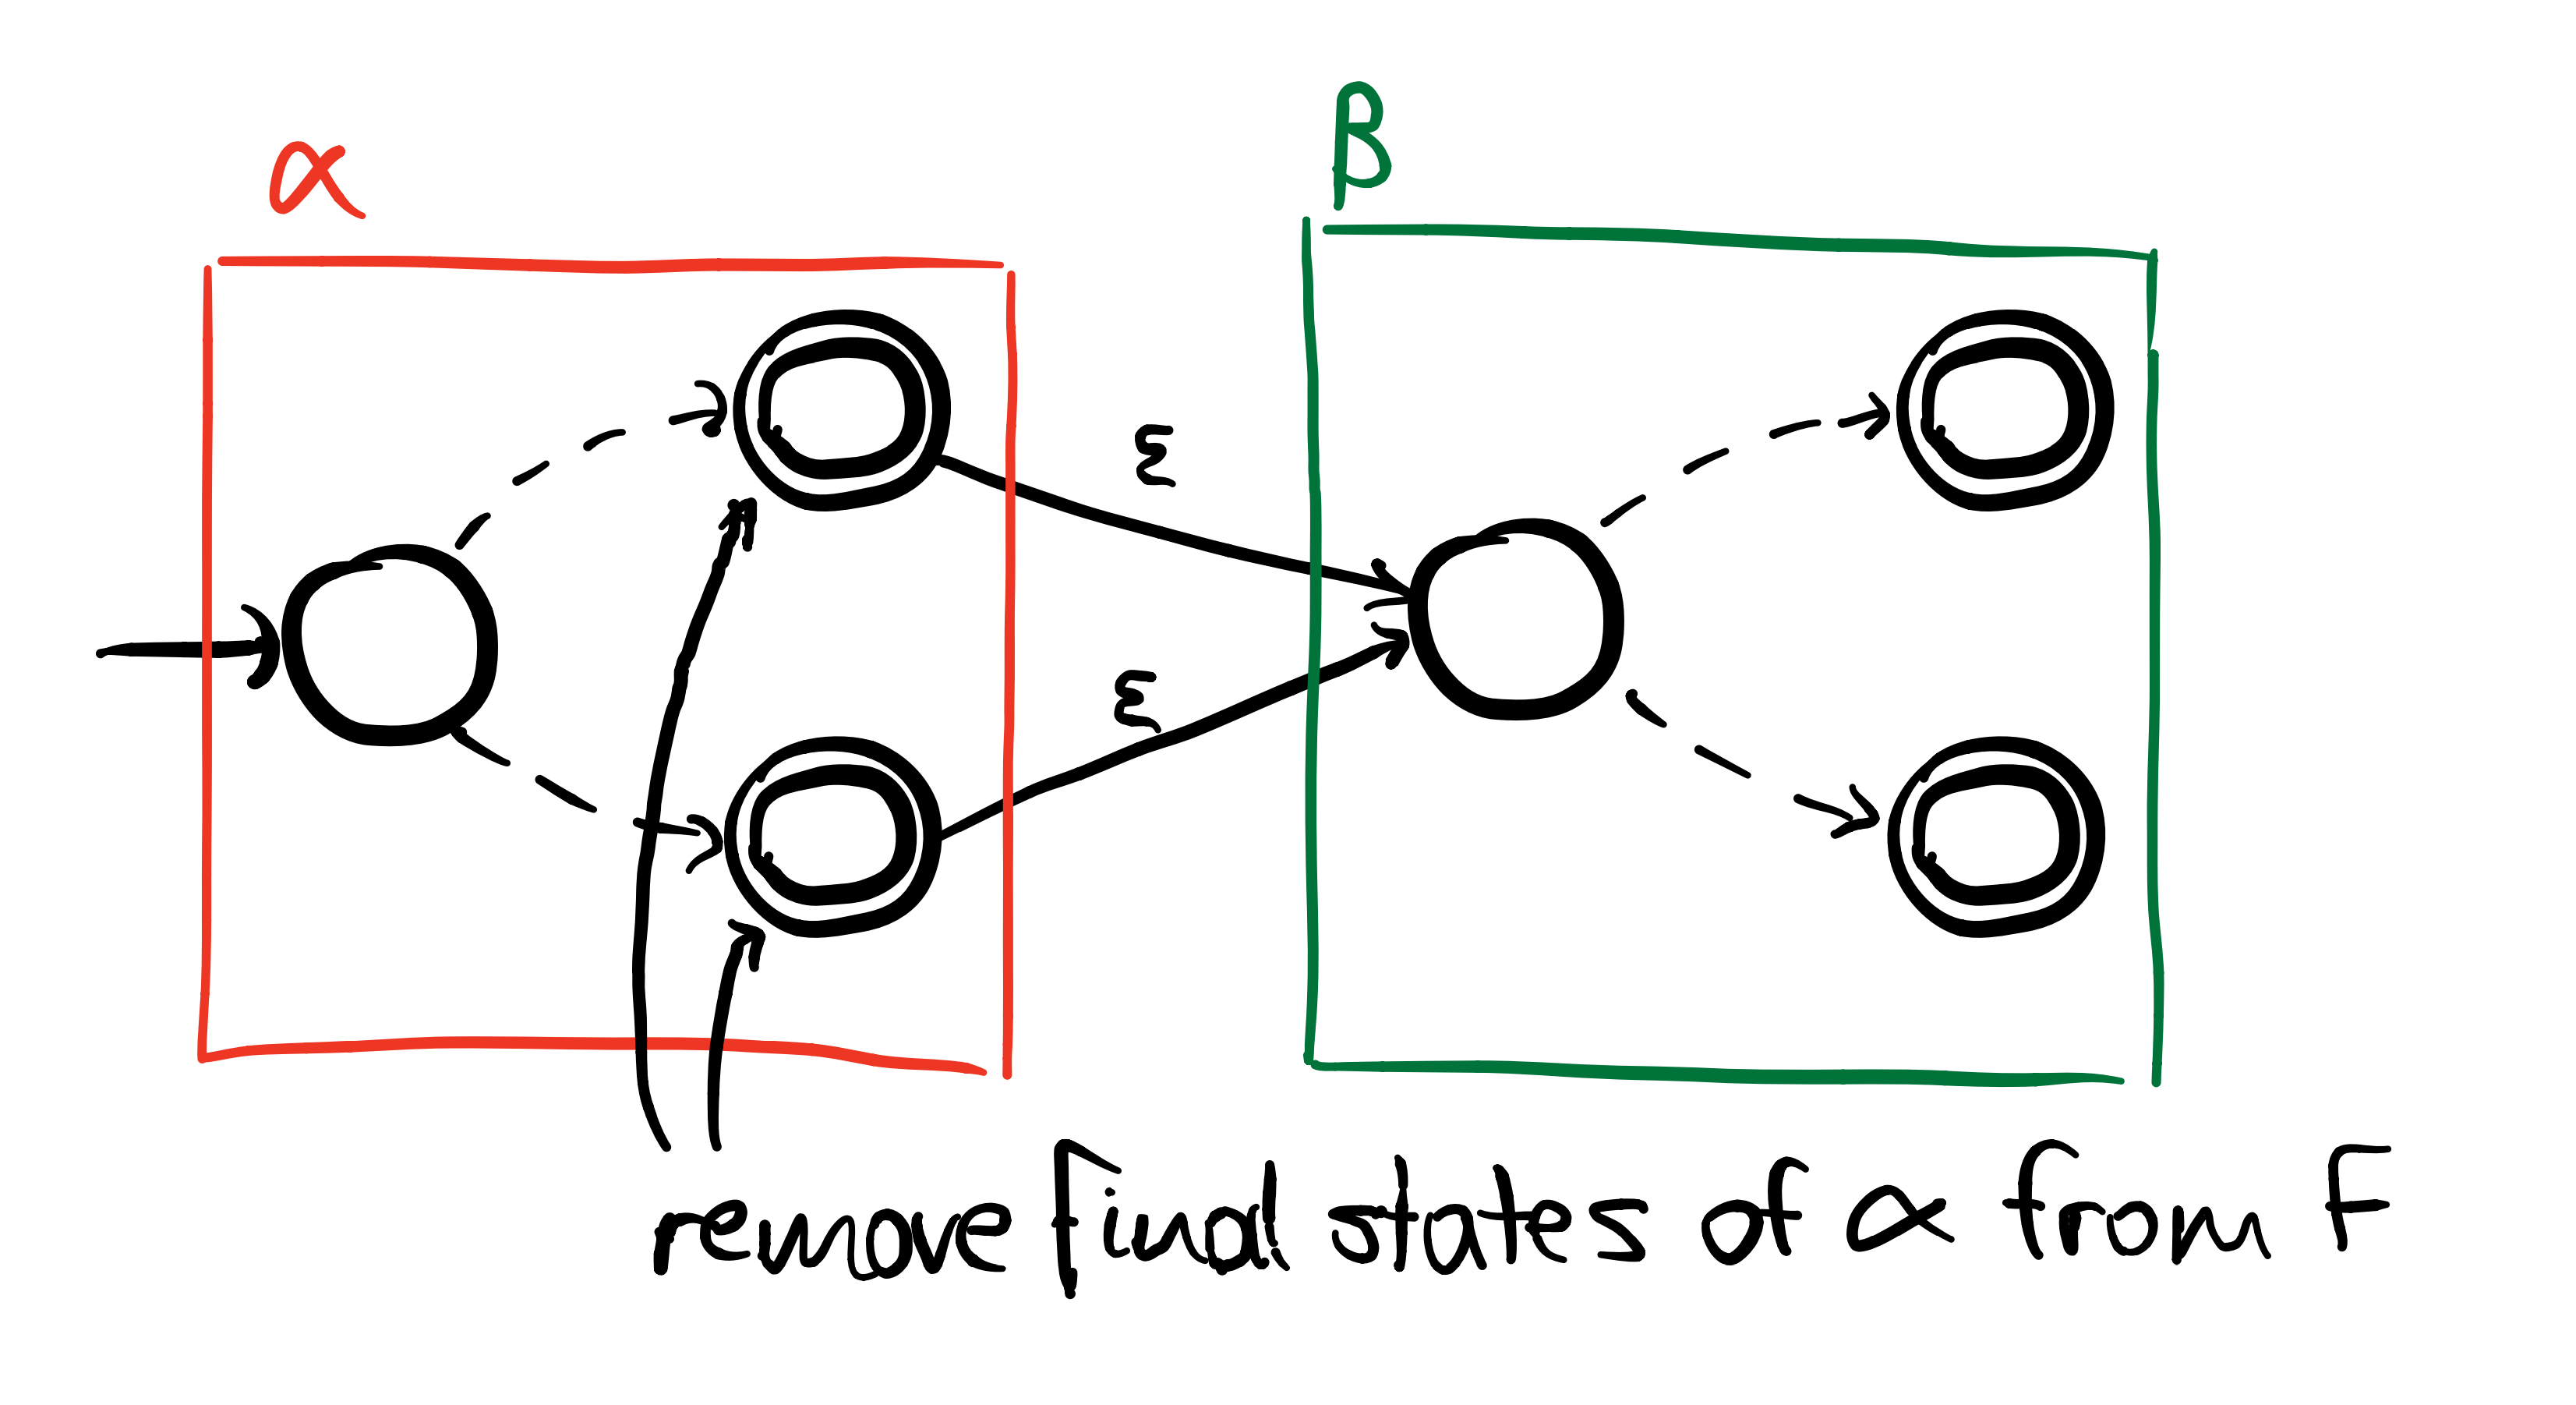
\includegraphics[width=8cm]{materials/images/regex_to_nfa_concatenation.png}
    \end{columns}
\end{frame}

\begin{frame}{Regex $\to$ $\epsilon$-NFA (Kleene)}
    \begin{columns}
        \column{0.1\textwidth}
        $\alpha \mid \beta$
        \column{0.6\textwidth}
        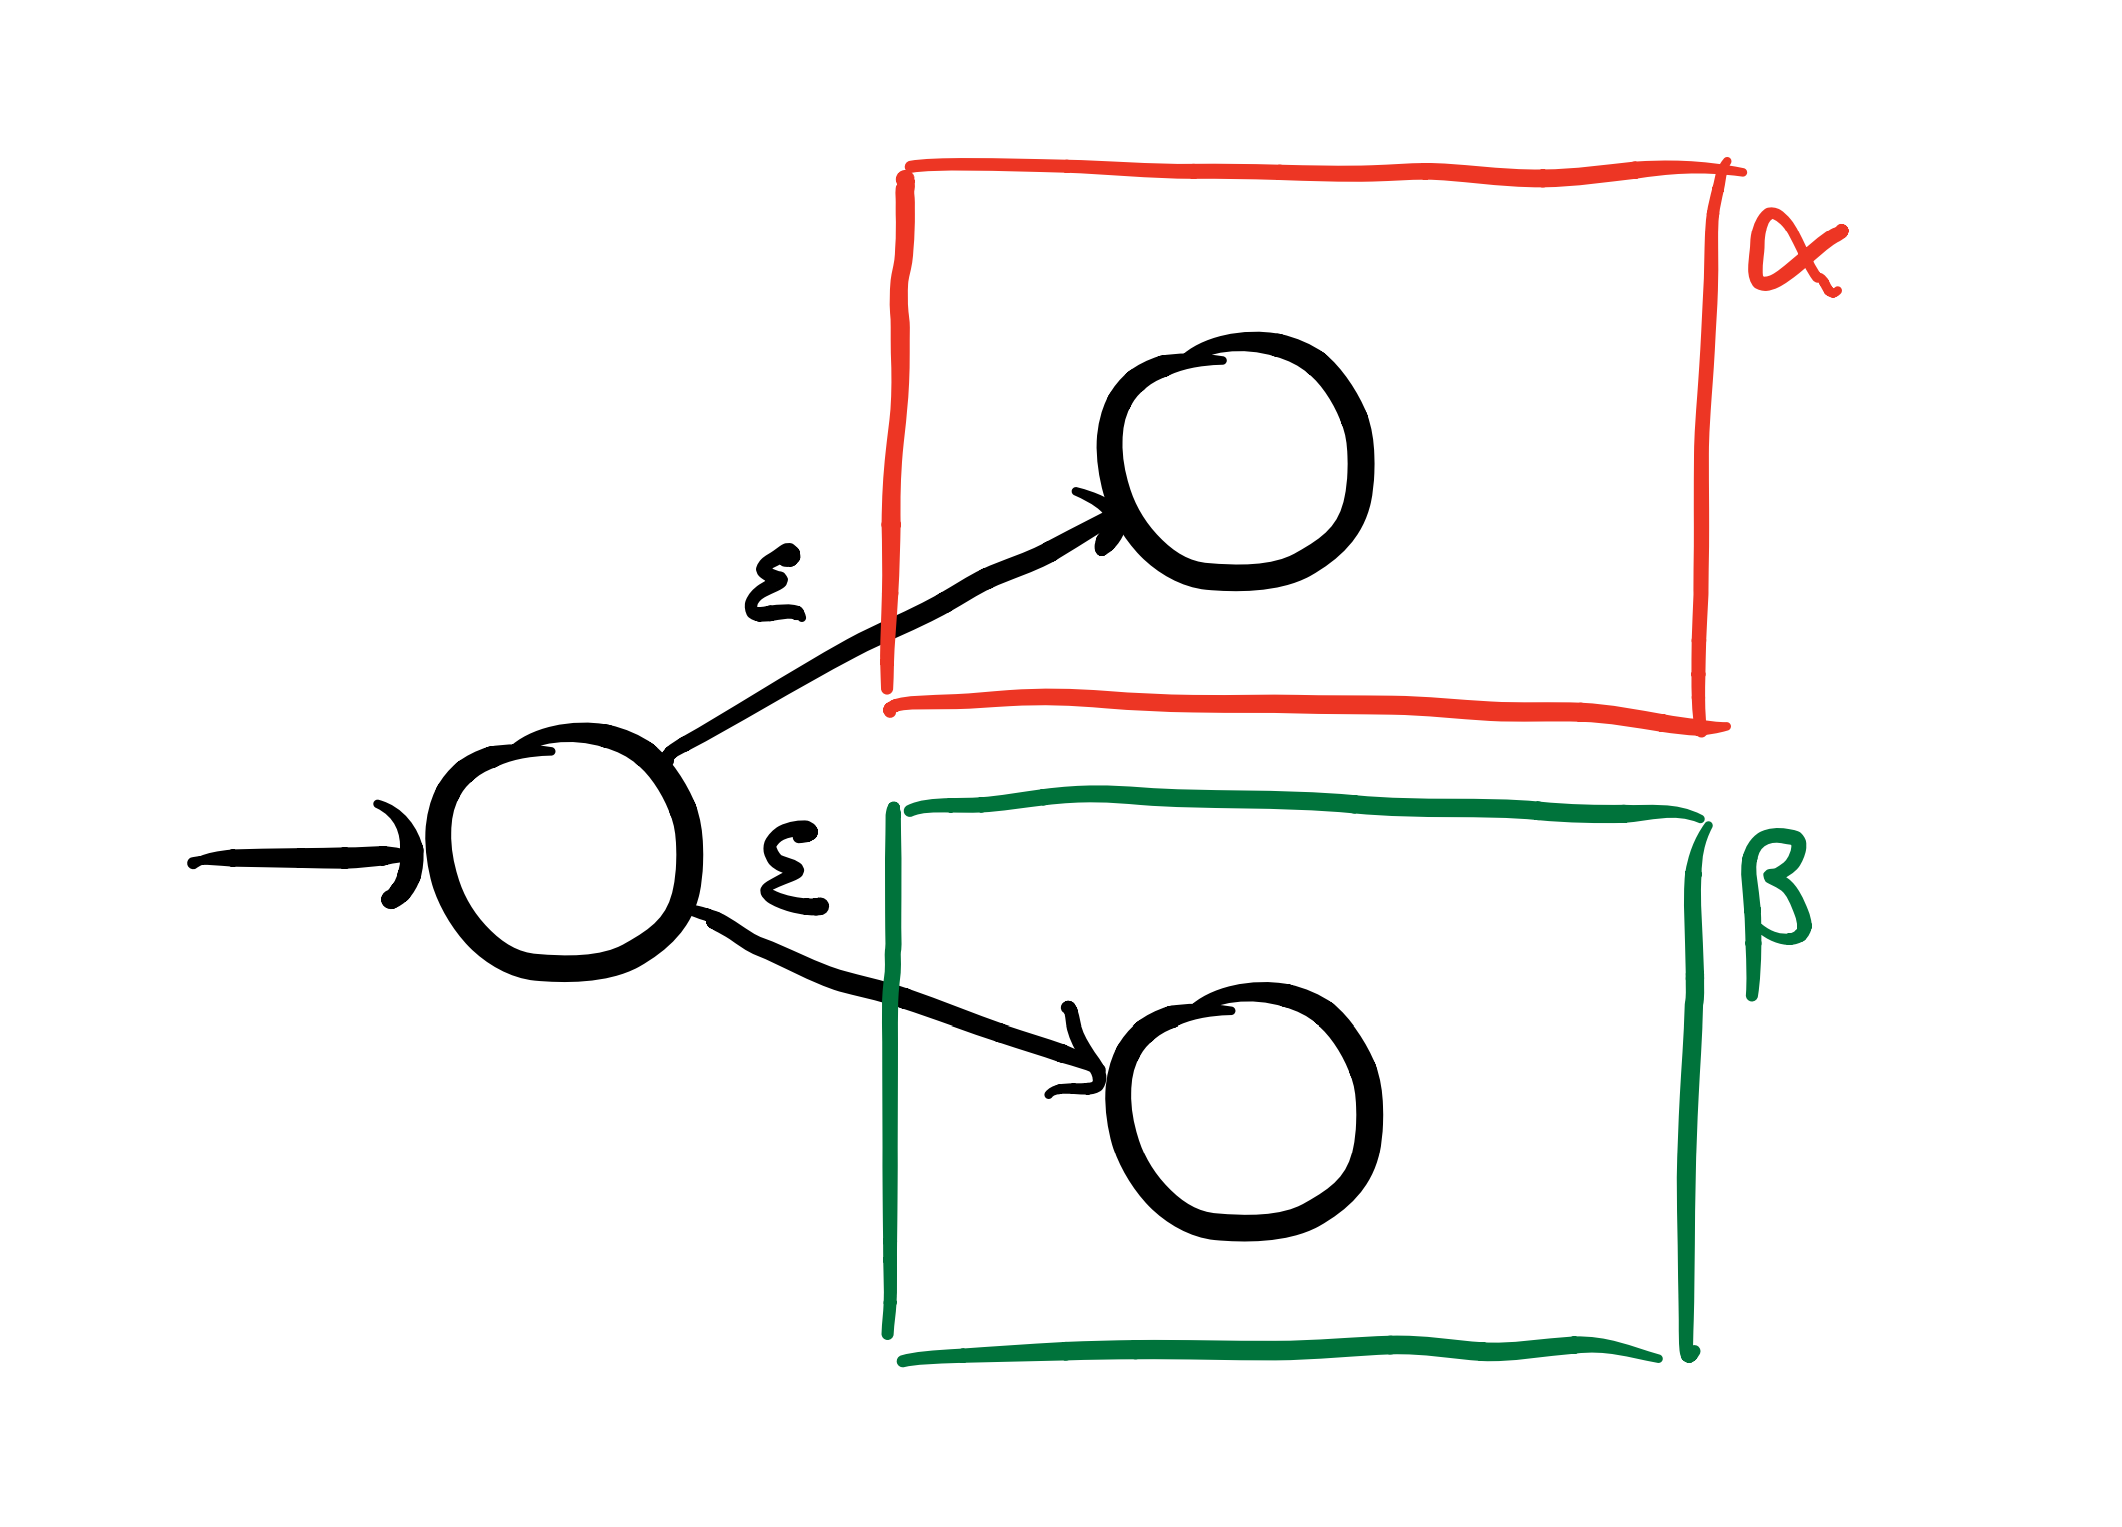
\includegraphics[width=5cm]{materials/images/regex_to_nfa_alternative.png}
    \end{columns}\pause
    \begin{columns}
        \column{0.1\textwidth}
        $\alpha^*$
        \column{0.6\textwidth}
        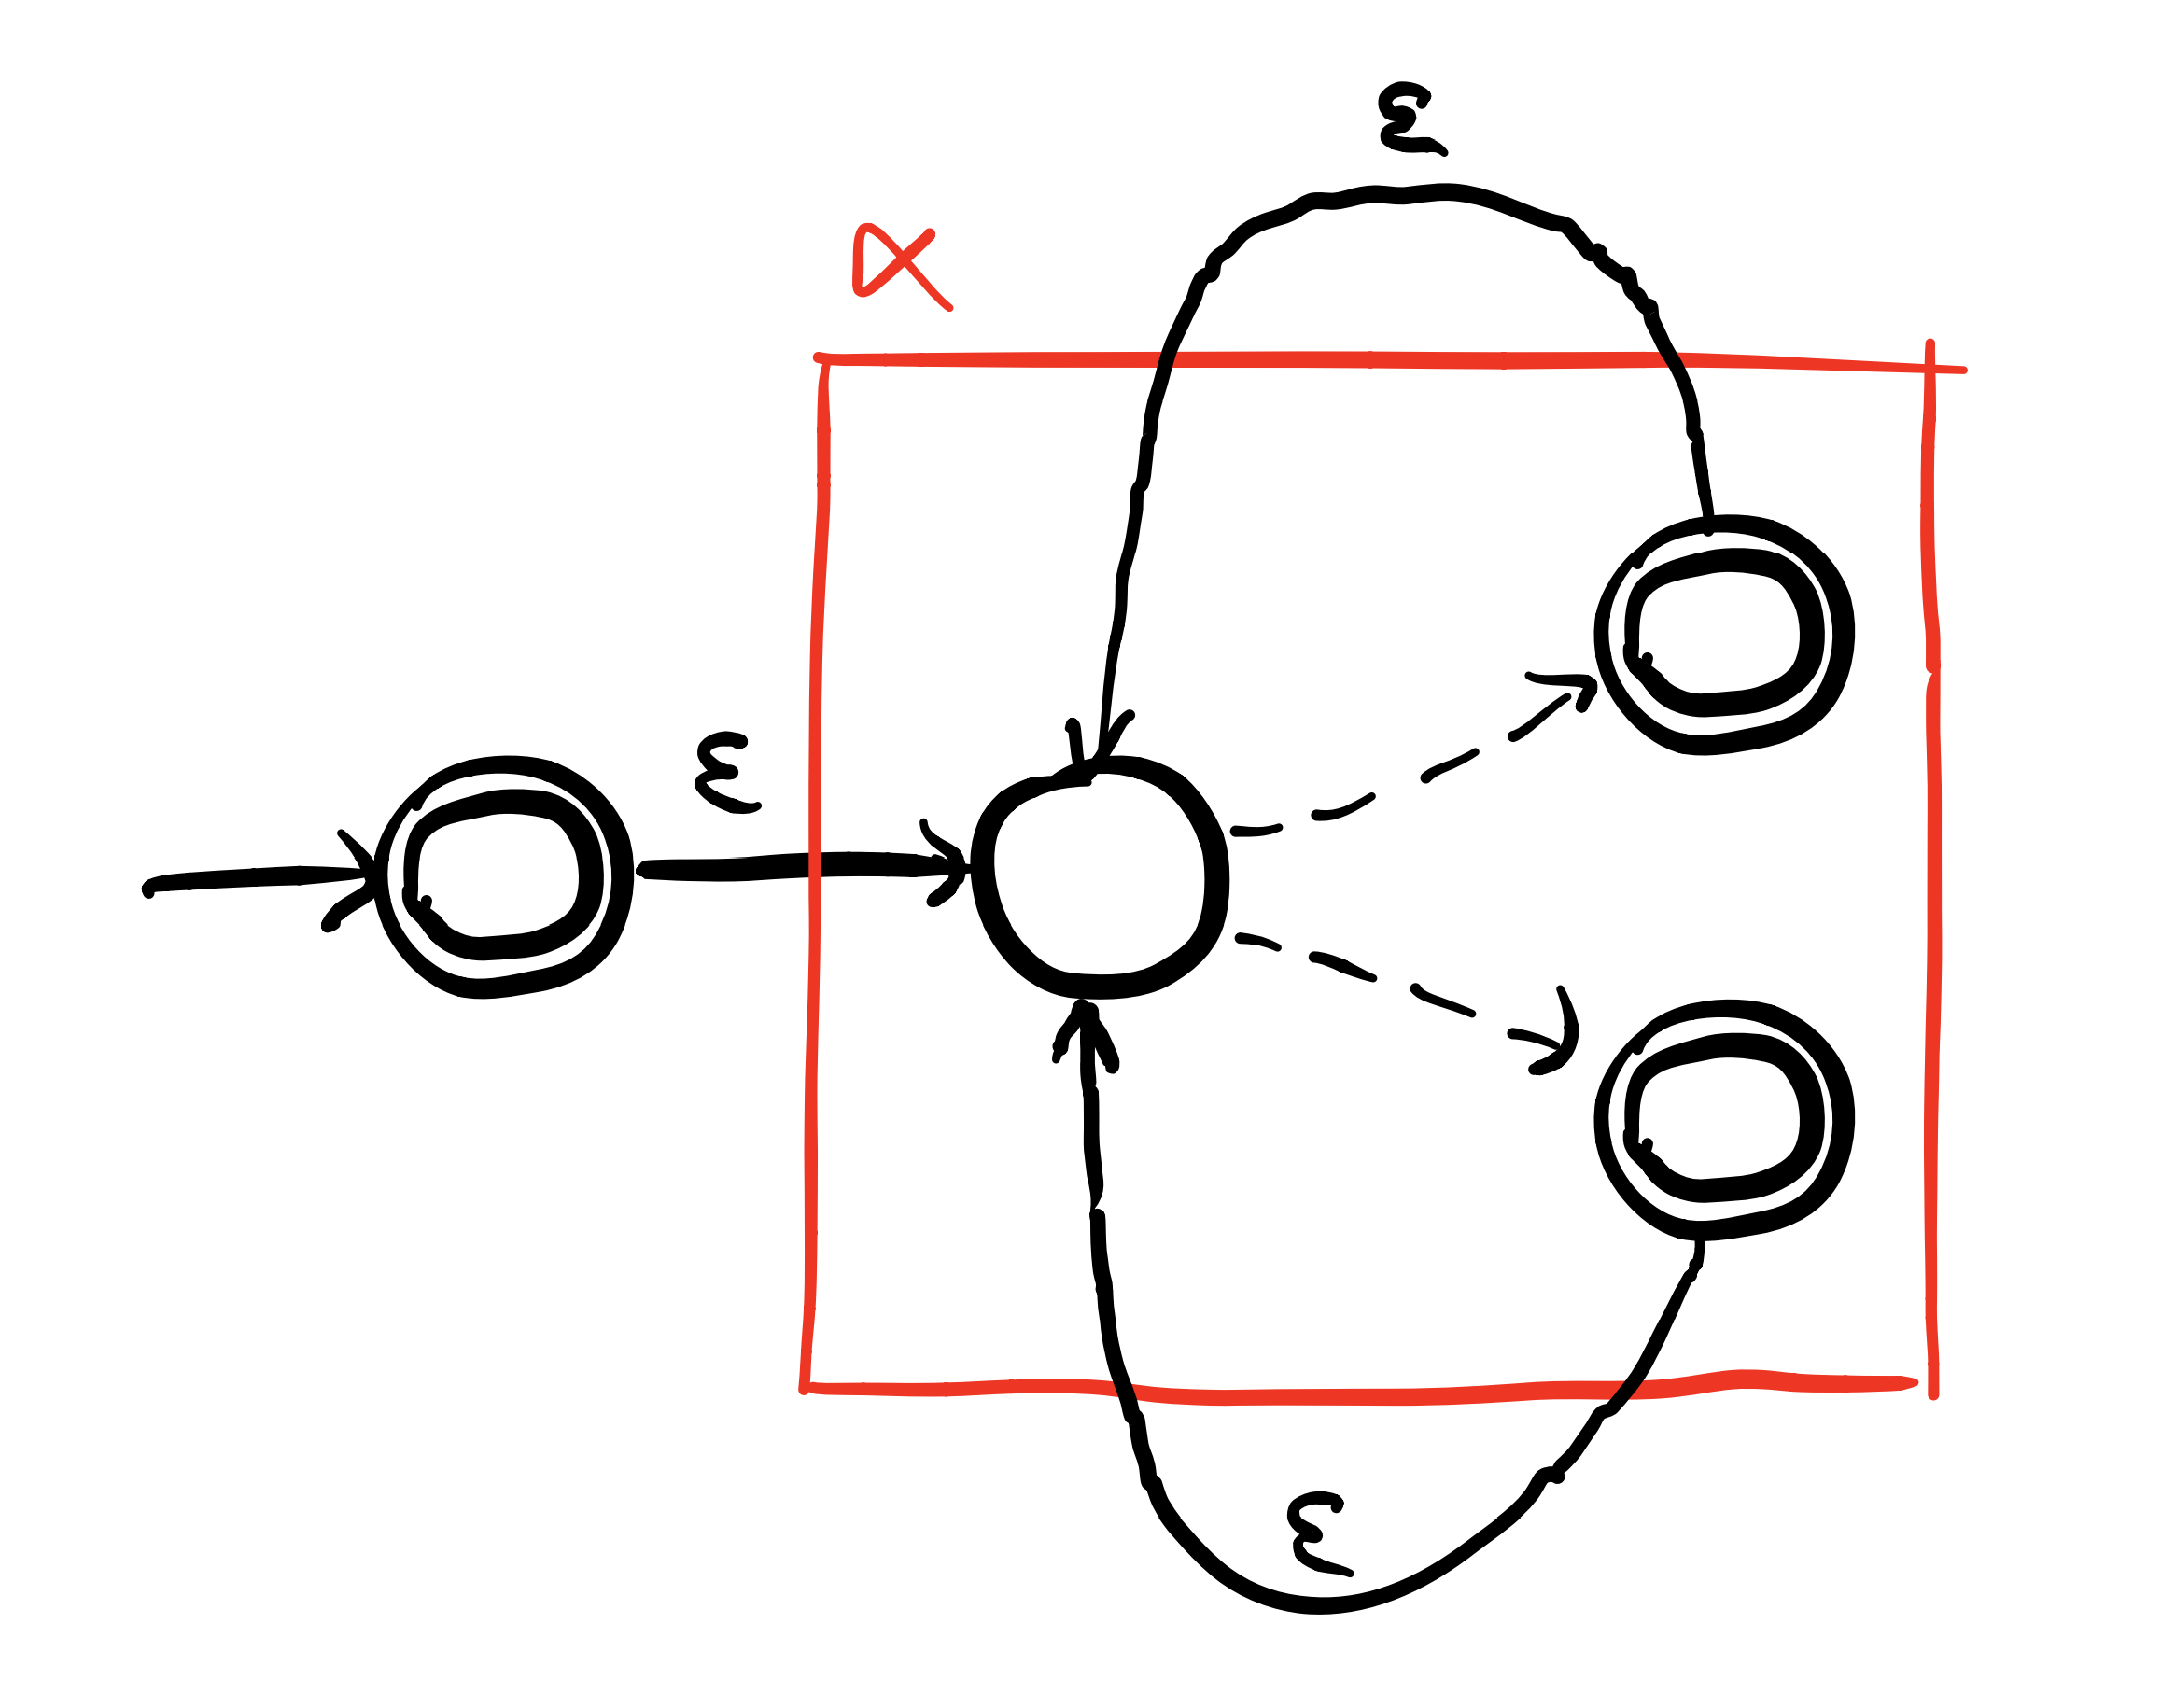
\includegraphics[width=5.5cm]{materials/images/regex_to_nfa_repetition.png}
    \end{columns}
\end{frame}

\subsection{DFA/NFA $\to$ Regex (Kleene)}

\begin{frame}{DFA/NFA $\to$ Regex (Kleene)}
    Given $M = (Q, \Sigma, \delta, q_1, F)$ with $Q = \{q_1, \dots, q_n\}$ define
    \begin{align*}
        R_{ij}^k = \{w \in \Sigma^* \mid &\text{ input } w \text{ transitions from } q_i \text{ to } q_j \\
        &\text{ and all states in between have an index  } \leq k\}.
    \end{align*}\pause
    Idea: for all $i, j \in [n]$ and $k \in [n]_0$\par
    a regex $\alpha_{ij}^k$ can be constructed with $L(\alpha_{ij}^k) = R_{ij}^k$.
\end{frame}

\begin{frame}{DFA/NFA $\to$ Regex (Kleene)}
    Induction over $k$.
    \begin{itemize}
        \item $k = 0$:\pause\ Let
            \begin{align*}
                R_{ij}^0 &= \begin{cases}
                    \{a \in \Sigma \mid \delta(q_i, a) = q_j\} & i \neq j \\
                    \{a \in \Sigma \mid \delta(q_i, a) = q_j\} \cup \{\epsilon\} & i = j
                \end{cases}\pause \\
                \alpha_{ij}^0 &= \begin{cases}
                    a_1 \mid \dots \mid a_l & i \neq j \\
                    a_1 \mid \dots \mid a_l \mid \epsilon & i = j
                \end{cases}
            \end{align*}\pause
            where $\{a_1, \dots, a_l\} = \{a \in \Sigma \mid \delta(q_i, a) = q_j\}$.\pause
        \item $k \implies k + 1$:\pause
            \begin{align*}
                R_{ij}^{k+1} &= R_{ij}^k\pause \cup \r{R_{i(k+1)}^k (R_{(k+1)(k+1)}^k)^* R_{(k+1)j}^k} \\
                \onslide<8->{\alpha_{ij}^{k+1}} &\onslide<8->{= a_{ij}^k \mid a_{i(k+1)}^k (a_{(k+1)(k+1)}^k)^* a_{(k+1)j}^k.
                }
            \end{align*}
            \r{New paths using $q_{k+1}$ in terms of the already built subpaths.}
    \end{itemize}
    \onslide<9->{We now have, $L(M) = L(\alpha_{1i_1}^n \mid \dots \mid \alpha_{1i_r}^n)$ where $\{q_{i_1}, \dots, q_{i_r}\} = F$.}
\end{frame}

\subsection{Arden's Lemma}

\begin{frame}{Arden's Lemma}
    \begin{theorem}[Arden's Lemma for regular languages]
        Let $A, B, X$ be regular languages and $\epsilon \not\in A$, then:
        \begin{align*}
            X = AX \cup B \implies X = A^* B.
        \end{align*}
    \end{theorem}\pause
    \begin{theorem}[Arden's Lemma for regular expressions]
        Let $\alpha, \beta, X$ be regular expressions and $\epsilon \not\in L(\alpha)$, then:
        \begin{align*}
            X = \alpha X \mid \beta \implies X = \alpha^* \beta.
        \end{align*}
    \end{theorem}
\end{frame}

\section{Closure Properties}

\begin{frame}{Closure Properties}
    \begin{theorem}
        Given the regular languages $R, R_1, R_2$, then the following are also regular languages:\pause
        \begin{itemize}
            \item $R_1 R_2$\pause;
            \item $R_1 \cup R_2$\pause;
            \item $R^*$\pause;
            \item $\bar{R}$\pause;
            \item $R_1 \cap R_2$\pause; and
            \item $R_1 \setminus R_2$.
        \end{itemize}
    \end{theorem}
\end{frame}

\section{Pumping Lemma}

\begin{frame}{Pumping Lemma}
    \begin{lemma}[Pumping Lemma for regular languages]
        Let $R \subseteq \Sigma^*$ be regular.\pause\ Then there exists some $n > 0$ such that every $z \in R$ with $|z| \geq n$ can be decomposed into $z = uvw$\pause\ such that
        \begin{itemize}
            \item $v \neq \epsilon$\pause;
            \item $|uv| \leq n$\pause; and
            \item $\forall i \geq 0.\ uv^iw \in R$.
        \end{itemize}
    \end{lemma}\pause
    \r{A necessary condition for regular languages.}
\end{frame}

\begin{frame}{Pumping Lemma}
    \begin{example}[proof structure]
        Assume $L$ is regular.\par
        Let $n > 0$ be a Pumping Lemma number.\pause\par
        Choose $z \in L$ with $|z| \geq n$.\par
        Define $z = uvw$ with $v \neq \epsilon$ and $|uv| \leq n$.\pause\par
        Then, $\forall i \geq 0.\ uv^iw \in L$.\pause\par
        Now, use the last statement to find a contradiction.
    \end{example}
\end{frame}

\end{document}
